\section{Theoretical Analysis}
\label{sec:analysis}



\subsection{Node Analysis ($t<0$)}

In this particular section, the circuit is analysed in $t<0$, therefore, we can apply the usual node analysis, with no sinusoidal tensions in the voltage source Vs: for $t<0$ $v_s = Vs$.

\begin{figure}[h] \centering
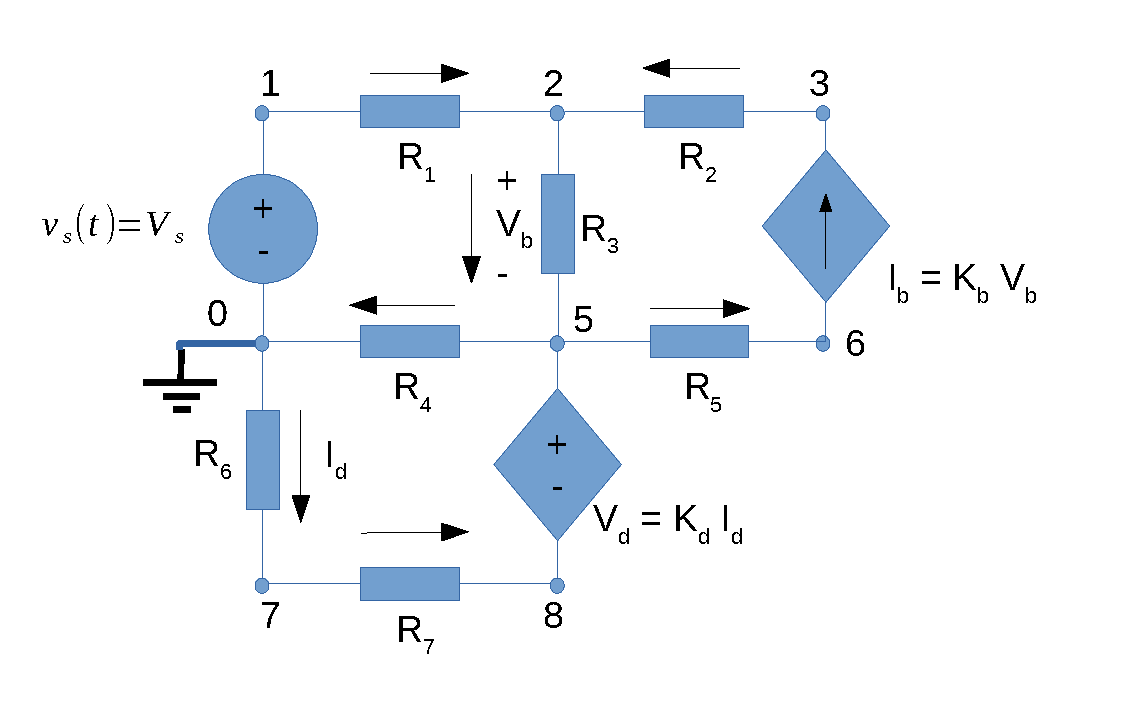
\includegraphics[width=0.5\linewidth]{t2-t1.pdf}
\caption{The circuit at $t<0$}
\label{fig2}
\end{figure}

Labels were assigned to identify nodes from zero to eight (no node four given in instructions), and directions to currents as seen in figure (\ref{fig2}), to then proceed with the node analysis.  We can, therefore, derive direct equations in terms of the voltage at these nodes.

For this procedure, one applies KCL (Kirchoff's Current Law), which states that the sum of currents leaving a node must be the same as the sum of currents entering a node. Because this kind of approach is only possible for the nodes which aren't directly connected to a terminal of a voltage source, it's crucial to find other equations to cover all the unknown variables of the system. In this case, it's important to consider factors like the voltage gain between two nodes separated by a voltage source: for example, from nodes 0 and 1, the terminals of $v_s$, we can take the equation: $V_1 = V_0 + V_s$. As $V_0$ is identified as the ground ($V_0 = 0V$) we're left with: $V_1 = V_s$.

Moreover, we can relate the currents associated with the current or voltage controlled sources with the nodes voltages, giving us two more equations, the nineth and tenth.

The equations are as follows:

\begin{equation} 
\begin{cases}

    Node\, 0: V_0 = 0 \\
    Node\, 1: V_1 = V_s \\
    Node\, 2: \frac{V_1 - V_2}{R_1} + \frac{V_3 - V_2}{R_2} - \frac{V_2 - V_5}{R_3} = 0 \\
    Node\, 3: -\frac{V_3 - V_2}{R_2} + I_b = 0 \\
    Node\, 5: V_5 - V_8 = V_d \\
    Node\, 6: \frac{V_5 - V_6}{R_5} - I_b = 0 \\
    Node\, 7: \frac{V_0 - V_7}{R_6} - \frac{V_7 - V_8}{R_7} = 0 \\
    Supernode\, 5-8: \frac{V_2 - V_5}{R_3} - \frac{V_5 - V_6}{R_5} + \frac{V_7 - V_8}{R_7} - \frac{V_5 - V_0}{R_4} = 0 \\
    I_d = \frac{V_0 - V_7}{R_6} \\
    I_b = K_b\,(V_2 - V_5) \\
    
\end{cases}
\label{eq:1}
\end{equation}


Note that, as there's no sinusoidal excitation ($v_s = constant$), the capacitor behaves like an open circuit and so the current $I_c$ is null and not included in the equations.


Using \textit{GNUOctave}, we computed the values of the node voltages by solving the system KCL equations above with matrixes. The currents in each branch were solved by aplication of Ohm's law ($I = \frac{V}{R}$) in each resistor, for example:

\begin{center}
  \begin{equation}
    I_1 = \frac{V_1 - V_2}{R_1}
  \end{equation} 
\end{center}


The value obtained are listed in the next tables:

\begin{table}[ht]
  \centering
  \begin{tabular}{|l|r|}
    \hline    
    {\bf Name} & {\bf Currents [A]} \\ \hline
    I1 & 2.3690260e-04\\\hline I2 & -2.4828279e-04\\\hline I3 & -1.1380187e-05\\\hline I4 & 1.2106395e-03\\\hline I5 & -2.4828279e-04\\\hline I6 & 9.7373690e-04\\\hline I7 & 9.7373690e-04\\\hline Ib & -2.4828279e-04\\\hline Id & 9.7373690e-04\\\hline Id & 0.0000000e+00\\\hline 
  \end{tabular}
  \caption{T2 1) Node Analysis Computation Results: Currents (A) computed using Ohm's law}
  \label{tab:nodeCurrents1}
\end{table}



\begin{table}[ht]
  \centering
  \begin{tabular}{|l|r|}
    \hline    
    {\bf Name} & {\bf Voltages [V]} \\ \hline
    V0 & 2.2132762e-16\\\hline V1 & 5.1850419e+00\\\hline V2 & 4.9415541e+00\\\hline V3 & 4.4258319e+00\\\hline V5 & 4.9770105e+00\\\hline V6 & 5.7290070e+00\\\hline V7 & -1.9765220e+00\\\hline V8 & -2.9546889e+00\\\hline Vb & -3.5456366e-02\\\hline Vd & 7.9316995e+00\\\hline 
  \end{tabular}
  \caption{T2 1) Node Analysis Computation Results: Voltages computed using KCL equations}
  \label{tab:nodeVoltages1}
\end{table}


\newpage

\subsection{Determining the Equivalent Resistance as Seen From Capacitor Terminals}

We start by turning off the independent voltage source, $v_s$, so we can study how the capacitor's charge disspates through the circuit. This is equivalent to connecting the capacitor in series with an equivalent resistor. This will be needed in the following section, where we'll be determining the differential equation that describes the original circuit.

Once we turn off $v_s$, it's crucial to make sure that there aren't discontinuous jumps in the circuits voltage, otherwise, we would obtain an infinite current as the capactior's equation states (voltage derivative):

\begin{center}
  \begin{equation}
    I_c(t) =  C \frac{dv(t)}{dt}
  \end{equation} 
\end{center}

Straightfowardly, the voltages at the capacitor's terminals must remain the same as before turning $v_s$ off. To do so, we can, theoretically, substitute the capacitor with an independent voltage source, $V_x$, where $V_x = V_6- V_8$, forcing the circuit's equations, while $v_s$ is off, to follow this boundary conditions.


\begin{figure}[h] \centering
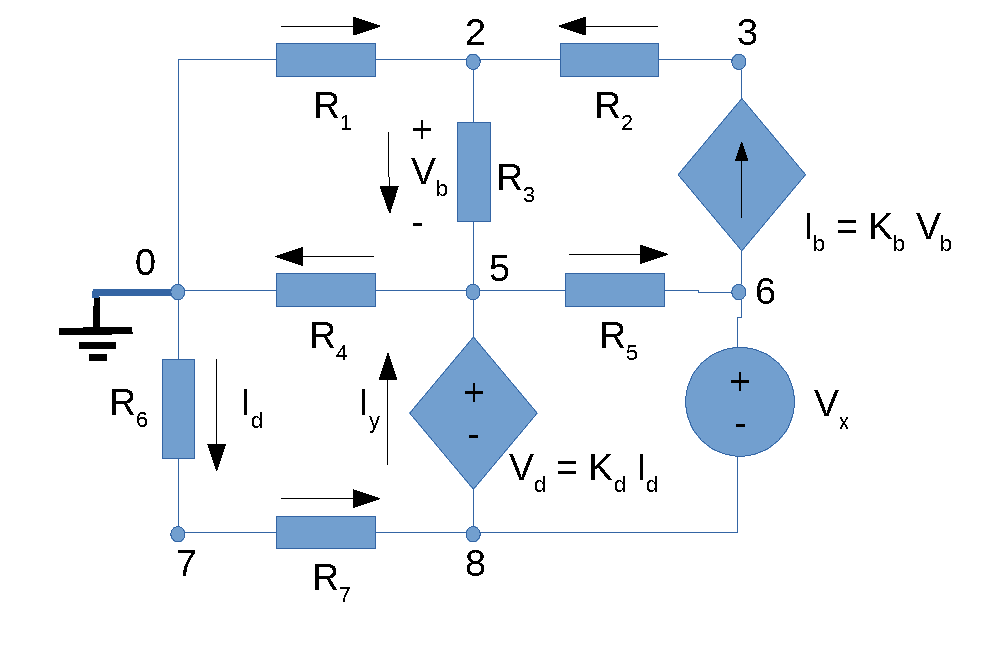
\includegraphics[width=0.5\linewidth]{t2-t2.pdf}
\caption{The circuit used to determine $R_{eq}$}
\label{fig3}
\end{figure}

Having done that, the circuit can once again be figured out using nodal analysis, as done in the previous section. However, instead of using supernode equations
(which would be problematic since we have a voltage source connected to another voltage source), we created two new variables, $I_x$ and $I_y$, which, of course,
require two new equations: these are now easily obtained since we can write KCL even in nodes connected to voltage sources. We end up with the equations:

\begin{equation} 
\begin{cases}

    Node\, 0: V_0 = 0 \\
    Node\, 2: \frac{V_0 - V_2}{R_1} + \frac{V_3 - V_2}{R_2} - \frac{V_2 - V_5}{R_3} = 0 \\
    Node\, 3: -\frac{V_3 - V_2}{R_2} + I_b = 0 \\
    Node\, 5.1: V_5 - V_8 = V_d \\
    Node\, 6.1: V_6 - V_8 = V_x \\
    Node\, 7: \frac{V_0 - V_7}{R_6} - \frac{V_7 - V_8}{R_7} = 0 \\
    Node\, 8: \frac{V_7 - V_8}{R_7} - I_y - I_x = 0 \\
    Node\, 5.2: I_y + \frac{V_2 - V_5}{R_3} - \frac{V_5 - V_6}{R_5} - \frac{V_5 - V_0}{R_4} = 0 \\
    Node\, 6.2: I_x + \frac{V_5 - V_6}{R_5} - I_b = 0 \\
    I_b = K_b\,(V_2 - V_5) \\
    V_d = K_d\,\frac{V_0 - V_7}{R_6}\\
    
\end{cases}
\label{eq:2}
\end{equation}

The nodal voltages resulting from these equations are compiled in the table \ref{tab:nodeVoltages2}; $I_x$ and $I_y$, aswell as the other currents obtained via
Ohm's Law are in \ref{tab:nodeCurrents2} and the equivalent resistor, $R_{eq}$, obtained via the equation $R_{eq} = \frac{V_x}{I_x}$, is in the table \ref{tab:Req}.

\begin{table}[h]
  \centering
  \begin{tabular}{|l|r|}
    \hline    
    {\bf Name} & {\bf Voltages [V]} \\ \hline
    V0 & -4.9144604e-32\\\hline V2 & -1.3014247e-15\\\hline V3 & -3.8742839e-15\\\hline V5 & -1.1245383e-15\\\hline V6 & 8.6836959e+00\\\hline V7 & 6.1145673e-16\\\hline V8 & 1.3292118e-15\\\hline Vb & -1.7688637e-16\\\hline Vd & -2.4537501e-15\\\hline 
  \end{tabular}
  \caption{Node Analysis Computation Results: Voltages computed using KCL equations}
  \label{tab:nodeVoltages2}
\end{table}


\begin{table}[h]
  \centering
  \begin{tabular}{|l|r|}
    \hline    
    {\bf Name} & {\bf Currents [A]} \\ \hline
    Ix & 2.8670509e-03\\\hline Iy & -2.8670509e-03\\\hline I1 & 1.2662274e-18\\\hline I2 & -1.2386447e-18\\\hline I3 & -5.6774006e-20\\\hline I4 & -2.7353981e-19\\\hline I5 & -2.8670509e-03\\\hline I7 & -7.1450436e-19\\\hline Ib & -1.2386447e-18\\\hline Id & -3.0123519e-19\\\hline 
  \end{tabular}
  \caption{Node Analysis Computation Results: Currents (A) computed using ohms law}
  \label{tab:nodeCurrents2}
\end{table}

\begin{table}[h]
  \centering
  \begin{tabular}{|l|r|}
    \hline    
    {\bf Name} & {\bf Currents [A]} \\ \hline
    Req & 3.0287903e+03\\\hline 
  \end{tabular}
  \caption{Equivalent Resistor as seen from the terminals of the capacitor}
  \label{tab:Req}
\end{table}



\clearpage
\subsection{Determining the Natural Solution for $V_6(t)$}

After reducing the rather complex circuit to a circuit with one voltage source, one resistor, $R_{eq}$, (between nodes with voltage $V_s$ and $V_6$, with this direction of voltage drop) and one capacitor, we can easily determine the natural solution on the system. More specifically, we can observe the behaviour of the capacitor, dissipating voltage through the resistors without any external excitation or driving force. 

To study this, we've worked out the voltage natural solution in node six ($V_{6n}$), in the interval [0, 20] ms.

For a simple RC series circuit (with a voltage source) we can derive the differential equation which describes the system. The natural solution is obtained by removing the voltage source: manipulating the differential equation yields: 

\begin{center}
  \begin{equation}
    V_{6n}(t) = K exp\left(-\frac{t}{RC}\right)
  \end{equation} 
\end{center}


,where $K$ is an integration constant.

To determine $K$, we need an initial condition, such as $V_6(t=0) = V_x$, determined in the last section. The final expression for $V_{6n}(t)$ is then:

\begin{center}
  \begin{equation}
    V_{6n}(t) = V_x exp\left(-\frac{t}{RC}\right)
  \end{equation} 
\end{center}



We used \textit{GNUOctave} to compute and plot $V_{6n}$ against time ([0, 20] ms), using a $1\mu s$ step, obtaining the following graphic:


\begin{figure}[h] \centering
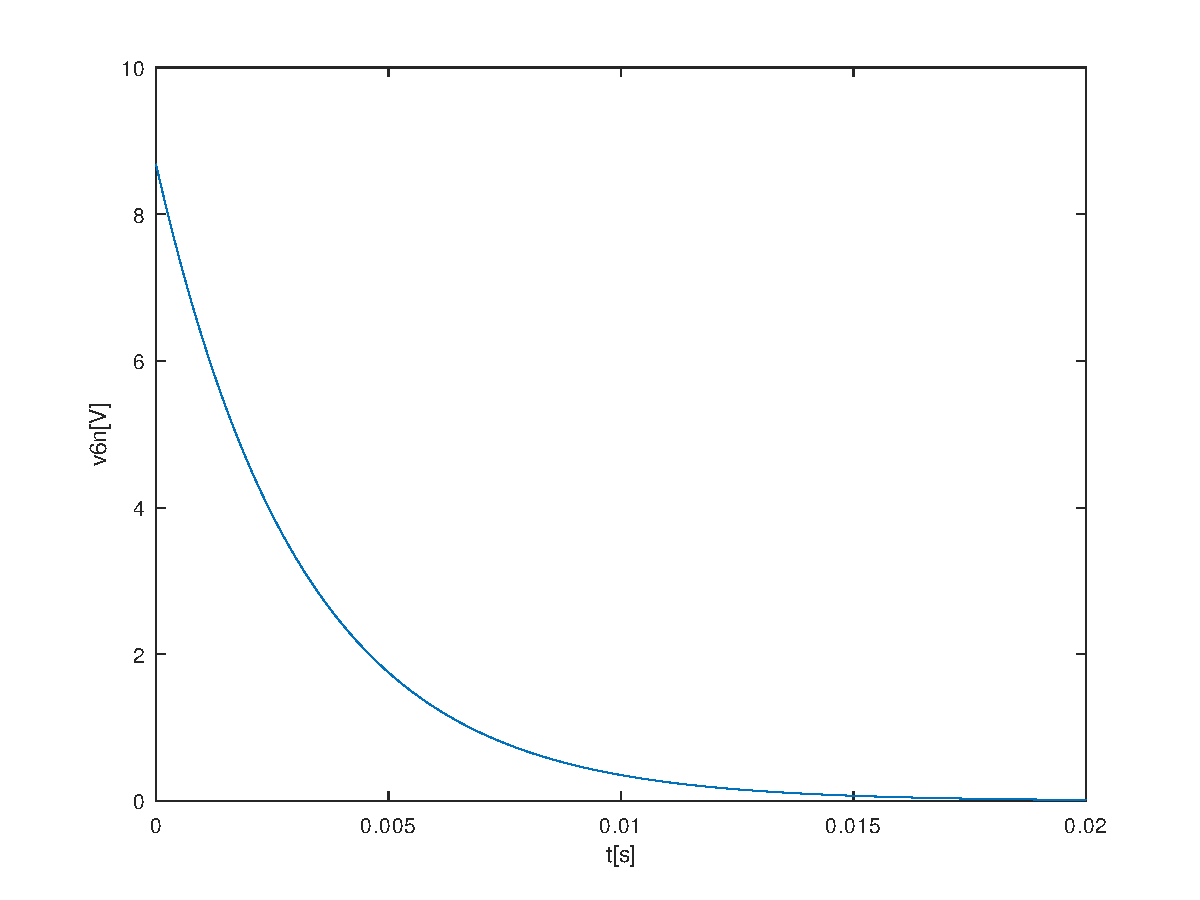
\includegraphics[width=0.6\linewidth]{../mat/t2-t3.pdf}
\caption{$V_{6n}(t)$, for t $\in$ [0, 20] ms}
\label{fig4}
\end{figure}


\newpage
\subsection{Determining the Forced Solution for $V_6(t)$}

For $t>0$, the independent voltage source, $v_s$, provides a sinusoidal excitation, which means the capacitor will now behave as expected and will dissipate current through it, $I_c$: this complicates the circuit tremendously. Working with sinusoidal functions in such big circuits requires a lot of computational work, thus, we will not do that. By transfering our voltages, currents and resistors to the complex domain, we can analyse the circuit and obtain complex solutions which, in the end, can be retrievable to the real world. The nodal analysis will be in everything similar to the previous sections, except for the fact that we substitute voltage $V_i$ for phasor $\tilde{V_i}$, current $I_i$ for $\tilde{I_i}$ and resistor $R_i$ for impedance $Z_i$.

\begin{figure}[h] \centering
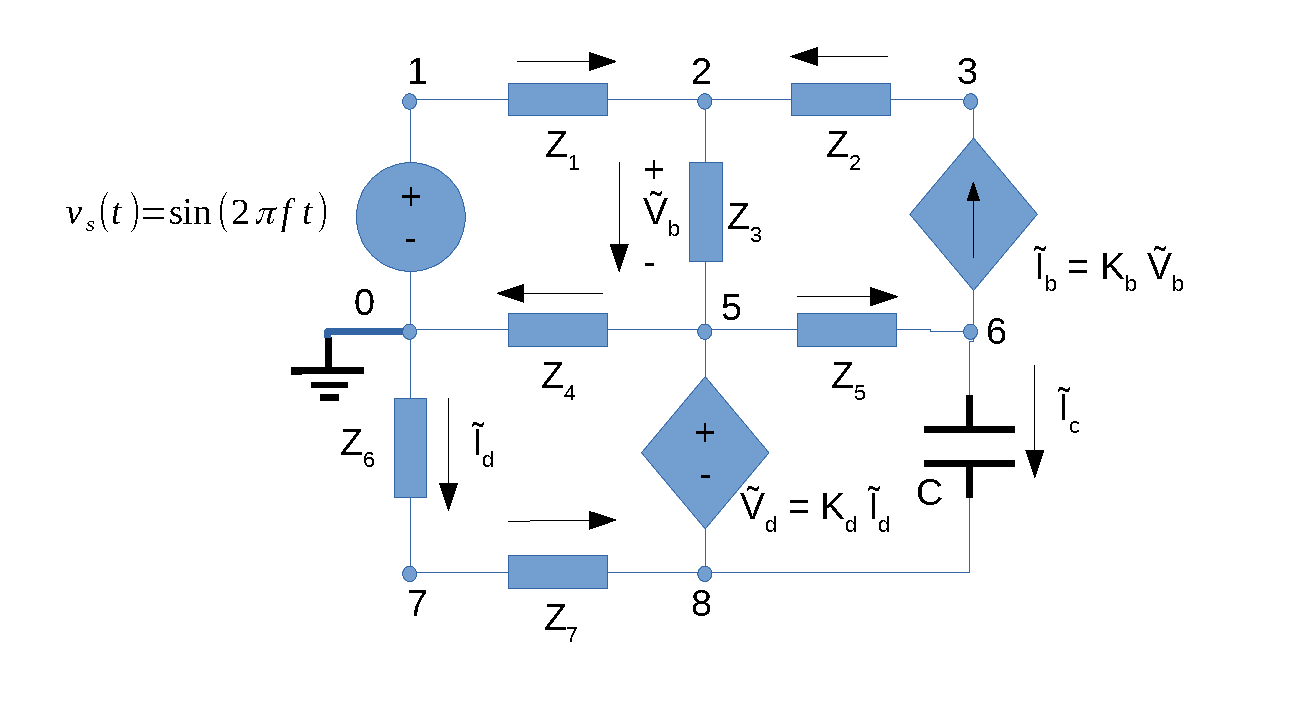
\includegraphics[width=0.6\linewidth]{t2-t3456.pdf}
\caption{The circuit for $t>0$, all variables in the complex domain}
\label{fig5}
\end{figure}

Moreover, the impedance of the resistor is equal to the resistor itself ($Z_i = R_i$) and the capacitor impedance can be written using the simple expression $Z_c = \frac{1}{j\omega C}$, in which $\omega = 2\pi f$ ($f =  1kHz$), the angular frequency of the source $v_s$ and C is the capacitance, a characteristic of the given capacitor. The equations to solve are then

\begin{equation} 
\begin{cases}

    Node\, 0: \tilde{V_0} = 0 \\
    Node\, 1: \tilde{V_1} - \tilde{V_0} = \tilde{V_s} \\
    Node\, 2: \frac{\tilde{V_1} - \tilde{V_2}}{Z_1} + \frac{\tilde{V_3} - \tilde{V_2}}{Z_2} - \frac{\tilde{V_2} - \tilde{V_5}}{Z_3} = 0 \\
    Node\, 3: -\frac{\tilde{V_3} - \tilde{V_2}}{Z_2} + \tilde{I_b} = 0 \\
    Node\, 5: \tilde{V_5} - \tilde{V_8} = \tilde{V_d} \\
    Node\, 6: \frac{\tilde{V_5} - \tilde{V_6}}{Z_5} - \tilde{I_b} - \tilde{I_c} = 0 \\
    Node\, 7: \frac{\tilde{V_0} - \tilde{V_7}}{Z_6} - \frac{\tilde{V_7} - \tilde{V_8}}{Z_7} = 0 \\
    Supernode\, 5-8: \frac{\tilde{V_2} - \tilde{V_5}}{Z_3} - \frac{\tilde{V_5} - \tilde{V_6}}{Z_5} + \frac{\tilde{V_7} - \tilde{V_8}}{Z_7} - \frac{\tilde{V_5} - \tilde{V_0}}{Z_4} + \tilde{I_c}= 0 \\
    %Supernode\, 0-1: \frac{\tilde{V_1} - \tilde{V_2}}{Z_1} + \frac{\tilde{V_0} - \tilde{V_7}}{Z_6} - \frac{\tilde{V_5} - \tilde{V_0}}{Z_4} = 0 \\
    \tilde{I_b} = K_b\,(\tilde{V_2} - \tilde{V_5}) \\
    \tilde{V_d} = K_d\,\frac{\tilde{V_0} - \tilde{V_7}}{Z_6}\\
    \tilde{I_c} = j 2\pi f C  (\tilde{V_6} - \tilde{V_8})\\
    \tilde{V_s} = 1 \\
    
\end{cases}
\label{eq:phasors}
\end{equation}

\begin{table}[h]
  \centering
  \begin{tabular}{|l|r|}
    \hline    
    {\bf Name} & {\bf Voltages [V]} \\ \hline
    V0real & -2.7665952e-17\\\hline V1real & 1.0000000e+00\\\hline V2real & 9.5304035e-01\\\hline V3real & 8.5357688e-01\\\hline V5real & 9.5987855e-01\\\hline V6real & -5.6551340e-01\\\hline V7real & -3.8119691e-01\\\hline V8real & -5.6984862e-01\\\hline 


V0imag & -2.4572302e-32\\\hline V1imag & 0.0000000e+00\\\hline V2imag & 5.8138780e-16\\\hline V3imag & 1.8224151e-15\\\hline V5imag & 4.9606606e-16\\\hline V6imag & -8.5097837e-02\\\hline V7imag & -1.9700289e-16\\\hline V8imag & -2.9449826e-16\\\hline 
  \end{tabular}
  \caption{Node Analysis Computation Results: Voltages computed using KCL equations}
  \label{tab:nodeVoltages4}
\end{table}




\newpage
\subsection{Determining the Final Total Solution for $V_6(t)$}

The final solution for node 6, $V_6(t)$, is obtained by summing its natural and forced solutions. We know that the forced solution will oscillate with the same frequency of the source $v_s$, but we don't know its amplitude yet. Well, that's exatly why we did what we did in the previous section. Since $v_s$ is a sine wave, we want $V_{6f}(t)$ to be a sine wave aswell, so we know we will have to extract the imaginary part of whatever expression we obtain. That expression is as follows

\begin{center}
  \begin{equation}
    V_{6f}(t) = (V6real + j\,V6imag)\, e^{j\omega t}
  \end{equation} 
\end{center}

Plotting $v_s(t)$ and $V_6(t)$, we end up with

\begin{figure}[h] \centering
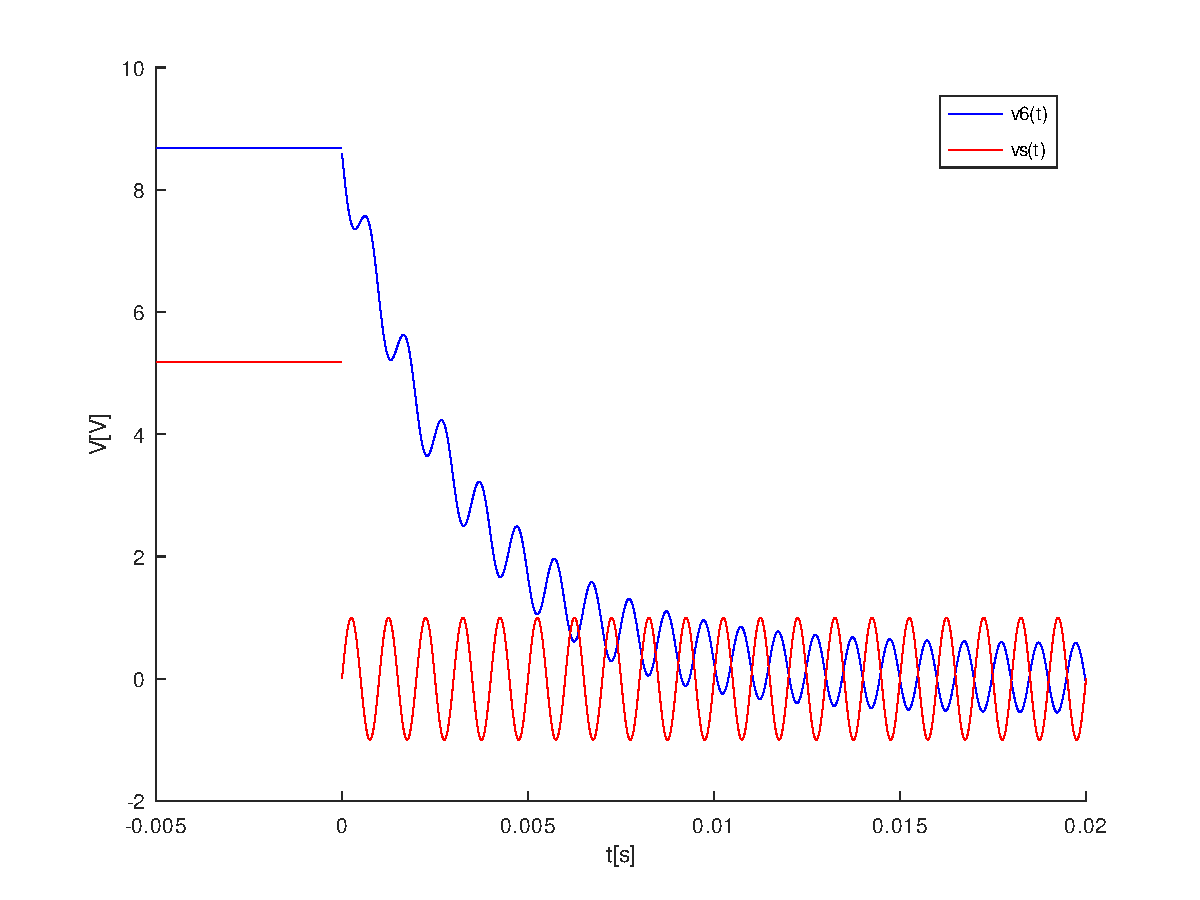
\includegraphics[width=0.6\linewidth]{../mat/t2-t5.pdf}
\caption{Voltage of $V_6$ and of the stimulus (V) vs. Time ($\in [0, 20]ms$) - Transient Analysis of the Original Circuit with a Forced Frequency of 1kHz}
\label{cfergter}
\end{figure}



\newpage

\subsection{Frequency analysis}

In this section, we analyse the frequency responses of $V_c(f) = V_6(f) - V_8(f)$ and $V_6(f)$, aswell as the behaviour of the source when we vary the frequency from 0.1 Hz to 1 MHz. This is usually done using a logarithmic scale for the frequency (base 10). We will plot the magnitude expressed in decibel (dB), a unit designed to easily give a human understanding to its value, since this circuit could, for example, be used in an amplifier, aswell as the phase expressed in degrees. Well, so far, every exercise was done using numeric computation, which provides less error, but this cannot be done here, since the nodal analysis requires every variable to be dependent on the frequency, $f$, otherwise, we would need milions of matrices... We call this symbolic computation. After running the same procedure as we did for subsection 4, even using those equations, we of course end up with nodal voltages, this time dependent on the frequency, $V_i(f)$. To do a bode plot, it is necessary to have a transfer function that depends on a variable, usually called $s$. $s$, in this case, is just $j \times f$, and this is very convenient since everywhere that $f$ appears in a given nodal voltage, is in its imaginary part. We therefore end up with an expression for $V_i(f)$ whose numerator and denominator is a polinomial in terms of $s$. Well, it's exactly in this form ([numerator denominator]) that transfer functions are written in $GNUOctave$, so we are done. All that remains is actually plotting the results, but this is done simply using the $bode$ command.

\begin{figure}[h] \centering
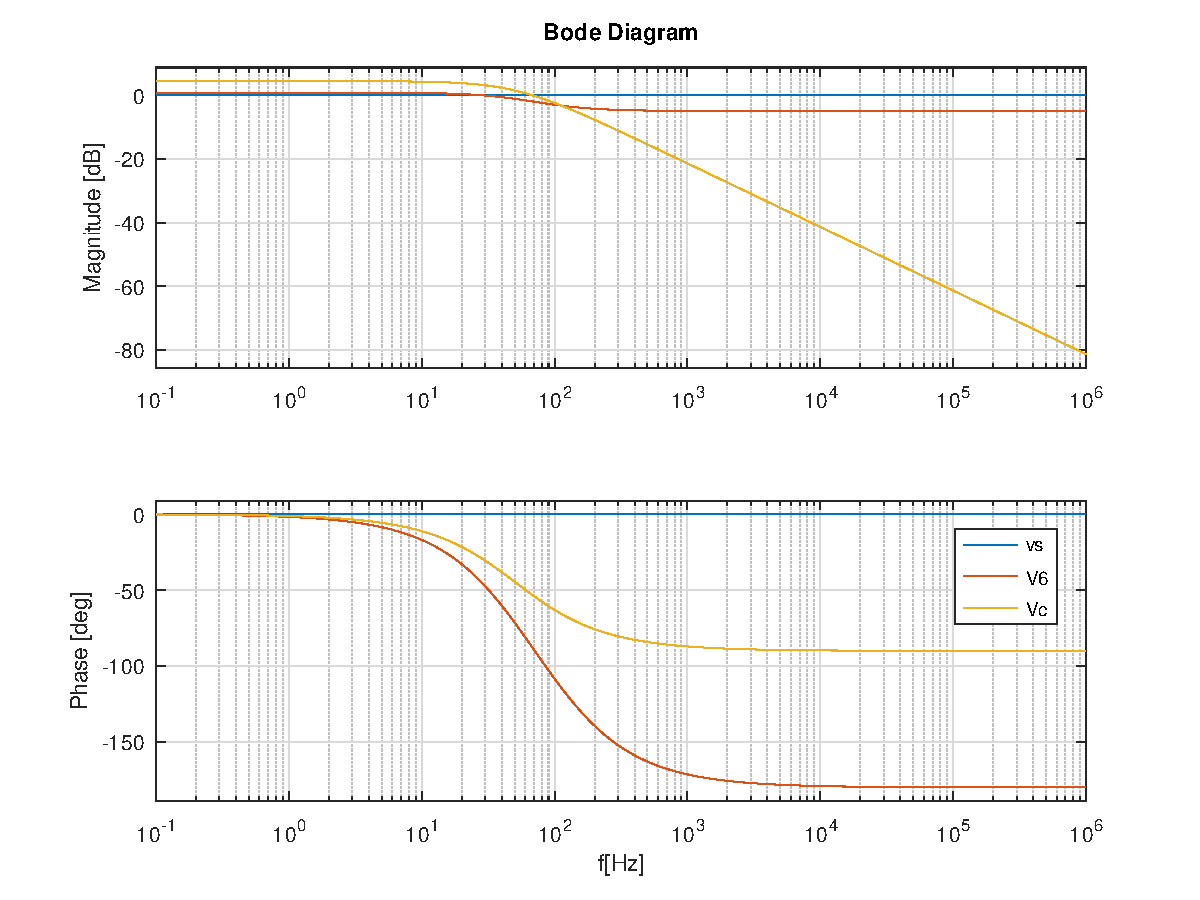
\includegraphics[width=0.95\linewidth]{../mat/t2-t6.pdf}
\caption{Bode plots for $v_s$, $V_c$ and $V_6$, f $\in$ [0.1, $10^6$] Hz}
\label{cfergter}
\end{figure}

The first thing that the reader might notice is that the amplitude of $v_s$ is always zero. This happens because $v_s$ is the voltage source, so it mantains its amplitude constant throughout frequency changes, unlike $V_6$. It is zero because the amplitude would be 1 in Volts, but, transforming the units into dB, we have to do the base 10 logarithm of the amplitude in Volts, which results in an amplitude in dB of zero.

As we can observe, all of the phases are 0 at $f=0.1Hz$ and then vary according to the frequency. The phase of $v_s$ is always 0, because its sine wave has no phase.